\documentclass{article}\usepackage[]{graphicx}\usepackage[]{color}
%% maxwidth is the original width if it is less than linewidth
%% otherwise use linewidth (to make sure the graphics do not exceed the margin)
\makeatletter
\def\maxwidth{ %
  \ifdim\Gin@nat@width>\linewidth
    \linewidth
  \else
    \Gin@nat@width
  \fi
}
\makeatother

\definecolor{fgcolor}{rgb}{0.345, 0.345, 0.345}
\newcommand{\hlnum}[1]{\textcolor[rgb]{0.686,0.059,0.569}{#1}}%
\newcommand{\hlstr}[1]{\textcolor[rgb]{0.192,0.494,0.8}{#1}}%
\newcommand{\hlcom}[1]{\textcolor[rgb]{0.678,0.584,0.686}{\textit{#1}}}%
\newcommand{\hlopt}[1]{\textcolor[rgb]{0,0,0}{#1}}%
\newcommand{\hlstd}[1]{\textcolor[rgb]{0.345,0.345,0.345}{#1}}%
\newcommand{\hlkwa}[1]{\textcolor[rgb]{0.161,0.373,0.58}{\textbf{#1}}}%
\newcommand{\hlkwb}[1]{\textcolor[rgb]{0.69,0.353,0.396}{#1}}%
\newcommand{\hlkwc}[1]{\textcolor[rgb]{0.333,0.667,0.333}{#1}}%
\newcommand{\hlkwd}[1]{\textcolor[rgb]{0.737,0.353,0.396}{\textbf{#1}}}%
\let\hlipl\hlkwb

\usepackage{framed}
\makeatletter
\newenvironment{kframe}{%
 \def\at@end@of@kframe{}%
 \ifinner\ifhmode%
  \def\at@end@of@kframe{\end{minipage}}%
  \begin{minipage}{\columnwidth}%
 \fi\fi%
 \def\FrameCommand##1{\hskip\@totalleftmargin \hskip-\fboxsep
 \colorbox{shadecolor}{##1}\hskip-\fboxsep
     % There is no \\@totalrightmargin, so:
     \hskip-\linewidth \hskip-\@totalleftmargin \hskip\columnwidth}%
 \MakeFramed {\advance\hsize-\width
   \@totalleftmargin\z@ \linewidth\hsize
   \@setminipage}}%
 {\par\unskip\endMakeFramed%
 \at@end@of@kframe}
\makeatother

\definecolor{shadecolor}{rgb}{.97, .97, .97}
\definecolor{messagecolor}{rgb}{0, 0, 0}
\definecolor{warningcolor}{rgb}{1, 0, 1}
\definecolor{errorcolor}{rgb}{1, 0, 0}
\newenvironment{knitrout}{}{} % an empty environment to be redefined in TeX

\usepackage{alltt}
\usepackage{amscd, amssymb, amsmath, verbatim, setspace}
\usepackage[left=1.0in, right=1.0in, top=1.0in, bottom=1.0in]{geometry}
\usepackage{mathrsfs}
\usepackage{listings}


\IfFileExists{upquote.sty}{\usepackage{upquote}}{}
\begin{document}
\begin{flushright}
Arif Ali\\
Math 611 Stochastic Simulation\\
Sept 15, 2016\\
\end{flushright}

\begin{center}
\LARGE\textbf{Homework 2}
  \end{center}
\section*{Exercise 1}
\begin{knitrout}
\definecolor{shadecolor}{rgb}{0.969, 0.969, 0.969}\color{fgcolor}\begin{kframe}
\begin{alltt}
\hlstd{transition_matrix} \hlkwb{=} \hlkwd{matrix}\hlstd{(}\hlkwd{c}\hlstd{(}\hlnum{0}\hlstd{,}\hlnum{1}\hlopt{/}\hlnum{25}\hlstd{,}\hlnum{0}\hlstd{,}\hlnum{0}\hlstd{,}\hlnum{0}\hlstd{,}\hlnum{0}\hlstd{,}\hlnum{1}\hlstd{,}\hlnum{8}\hlopt{/}\hlnum{25}\hlstd{,}\hlnum{4}\hlopt{/}\hlnum{25}\hlstd{,}\hlnum{0}\hlstd{,}\hlnum{0}\hlstd{,}\hlnum{0}\hlstd{,}
         \hlnum{0}\hlstd{,}\hlnum{16}\hlopt{/}\hlnum{25}\hlstd{,}\hlnum{12}\hlopt{/}\hlnum{25}\hlstd{,}\hlnum{9.25}\hlstd{,}\hlnum{0}\hlstd{,}\hlnum{0}\hlstd{,} \hlnum{0}\hlstd{,}\hlnum{0}\hlstd{,}\hlnum{9}\hlopt{/}\hlnum{25}\hlstd{,}\hlnum{12}\hlopt{/}\hlnum{25}\hlstd{,}\hlnum{16}\hlopt{/}\hlnum{25}\hlstd{,}\hlnum{0}\hlstd{,}
         \hlnum{0}\hlstd{,}\hlnum{0}\hlstd{,}\hlnum{0}\hlstd{,}\hlnum{4}\hlopt{/}\hlnum{25}\hlstd{,}\hlnum{8}\hlopt{/}\hlnum{25}\hlstd{,}\hlnum{1}\hlstd{,} \hlnum{0}\hlstd{,}\hlnum{0}\hlstd{,}\hlnum{0}\hlstd{,}\hlnum{0}\hlstd{,}\hlnum{1}\hlopt{/}\hlnum{25}\hlstd{,}\hlnum{0}\hlstd{),} \hlkwc{ncol} \hlstd{=} \hlnum{6}\hlstd{)}
\hlkwd{row.names}\hlstd{(transition_matrix)} \hlkwb{=} \hlnum{0}\hlopt{:}\hlnum{5}
\hlkwd{colnames}\hlstd{(transition_matrix)} \hlkwb{=} \hlnum{0}\hlopt{:}\hlnum{5}
\hlstd{transition_matrix}
\end{alltt}
\begin{verbatim}
##      0    1    2    3    4    5
## 0 0.00 1.00 0.00 0.00 0.00 0.00
## 1 0.04 0.32 0.64 0.00 0.00 0.00
## 2 0.00 0.16 0.48 0.36 0.00 0.00
## 3 0.00 0.00 9.25 0.48 0.16 0.00
## 4 0.00 0.00 0.00 0.64 0.32 0.04
## 5 0.00 0.00 0.00 0.00 1.00 0.00
\end{verbatim}
\end{kframe}
\end{knitrout}
In order to create the transition matrix, the following rules were set, at right urn with 0 black balls, the only possible position was to gain 1 and for right urn with 5 black balls, only option was to lose 1. In the other cases, to lose a black ball, the proportion of black balls in the right urn was multiplied by the proportion of white balls in the left urn. To gain a black ball, the proportion of white balls in the right urn was multiplied by the proportion of black balls in the left urn. For no gain, the two cases where a ball of the same color was pick were added.


Based on the matrix the probabilities are derived as the following (note we define $m=5$):

$p(i, i-1)=\frac{i^{2}}{m^{2}}$

$p(i,i+1)=\frac{(m-i)^{2}}{m^{2}}$

$p(i,i)=\frac{m^{2}-(m-i)^{2}-i^2}{m^2}=\frac{m^{2}-(m^2-2mi+i^2)-i^2}{m^2}=\frac{2mi-2i^{2}}{m^{2}}$

\section*{Exercise 2}
\subsubsection*{$p^{3}(1,3)$}
It's impossible to go from spot 1 to 3 within 3 steps: $p^{3}(1,3) = 0$

\subsubsection*{$p^{2}(1,4)$}
It's impossible to go from spot 1 to 4 within 2 steps: $p^{2}(1,4) = 0$

\subsubsection*{$p^3(1,0)$}
There are two possible ways to go from 1 to 0 within 3 steps: $p^3(1,0) = 0.6 + 0.6*0.4*0.6 = 0.744$
The first step is possible because once an enpoint is hit, the probability of staying at the endpoint is one.

\section*{Exercise 3}
\begin{knitrout}
\definecolor{shadecolor}{rgb}{0.969, 0.969, 0.969}\color{fgcolor}\begin{kframe}
\begin{alltt}
\hlstd{two_state_matrix} \hlkwb{=} \hlkwd{matrix}\hlstd{(}\hlkwd{c}\hlstd{(}\hlnum{0.3}\hlstd{,}\hlnum{0.6}\hlstd{,}\hlnum{0.7}\hlstd{,}\hlnum{0.4}\hlstd{),} \hlkwc{ncol} \hlstd{=} \hlnum{2}\hlstd{)}
\hlkwd{row.names}\hlstd{(two_state_matrix)} \hlkwb{=} \hlkwd{c}\hlstd{(}\hlstr{"H"}\hlstd{,} \hlstr{"M"}\hlstd{)}
\hlkwd{colnames}\hlstd{(two_state_matrix)} \hlkwb{=} \hlkwd{c}\hlstd{(}\hlstr{"H"}\hlstd{,} \hlstr{"M"}\hlstd{)}
\hlstd{two_state_matrix}
\end{alltt}
\begin{verbatim}
##     H   M
## H 0.3 0.7
## M 0.6 0.4
\end{verbatim}
\end{kframe}
\end{knitrout}
\section*{Exercise 4}
\subsection*{Part A}
\begin{knitrout}
\definecolor{shadecolor}{rgb}{0.969, 0.969, 0.969}\color{fgcolor}\begin{kframe}
\begin{alltt}
\hlstd{M} \hlkwb{=} \hlkwd{optimize}\hlstd{(}\hlkwc{f}\hlstd{=}\hlkwa{function}\hlstd{(}\hlkwc{x}\hlstd{)\{}\hlkwd{dbeta}\hlstd{(x,}\hlnum{2}\hlstd{,}\hlnum{2}\hlstd{)\},} \hlkwc{interval}\hlstd{=}\hlkwd{c}\hlstd{(}\hlnum{0}\hlstd{,}\hlnum{1}\hlstd{),}\hlkwc{maximum} \hlstd{=T)}\hlopt{$}\hlstd{objective}
\hlstd{x} \hlkwb{=} \hlkwa{NULL}
\hlstd{Nsim}\hlkwb{=}\hlnum{1e4}
\hlkwa{while} \hlstd{(}\hlkwd{length}\hlstd{(x)}\hlopt{<}\hlstd{Nsim)\{}
  \hlstd{y}\hlkwb{=}\hlkwd{runif}\hlstd{(Nsim}\hlopt{*}\hlstd{M)}
  \hlstd{x}\hlkwb{=}\hlkwd{c}\hlstd{(x,y[}\hlkwd{runif}\hlstd{(Nsim}\hlopt{*}\hlstd{M)}\hlopt{*}\hlstd{M}\hlopt{<}\hlkwd{dbeta}\hlstd{(y,}\hlnum{2}\hlstd{,}\hlnum{2}\hlstd{)])}
  \hlstd{\}}
\hlstd{x}\hlkwb{=}\hlstd{x[}\hlnum{1}\hlopt{:}\hlstd{Nsim]}

\hlkwd{hist}\hlstd{(x,} \hlkwc{breaks} \hlstd{=} \hlnum{40}\hlstd{,} \hlkwc{freq} \hlstd{= F,} \hlstr{"xlab"} \hlstd{=} \hlstr{"Accepted Values"}\hlstd{)}
\hlkwd{curve}\hlstd{(}\hlkwd{dbeta}\hlstd{(x,} \hlnum{2}\hlstd{,}\hlnum{2}\hlstd{),} \hlkwc{add} \hlstd{= T,} \hlkwc{col} \hlstd{=} \hlstr{"red"}\hlstd{)}
\end{alltt}
\end{kframe}
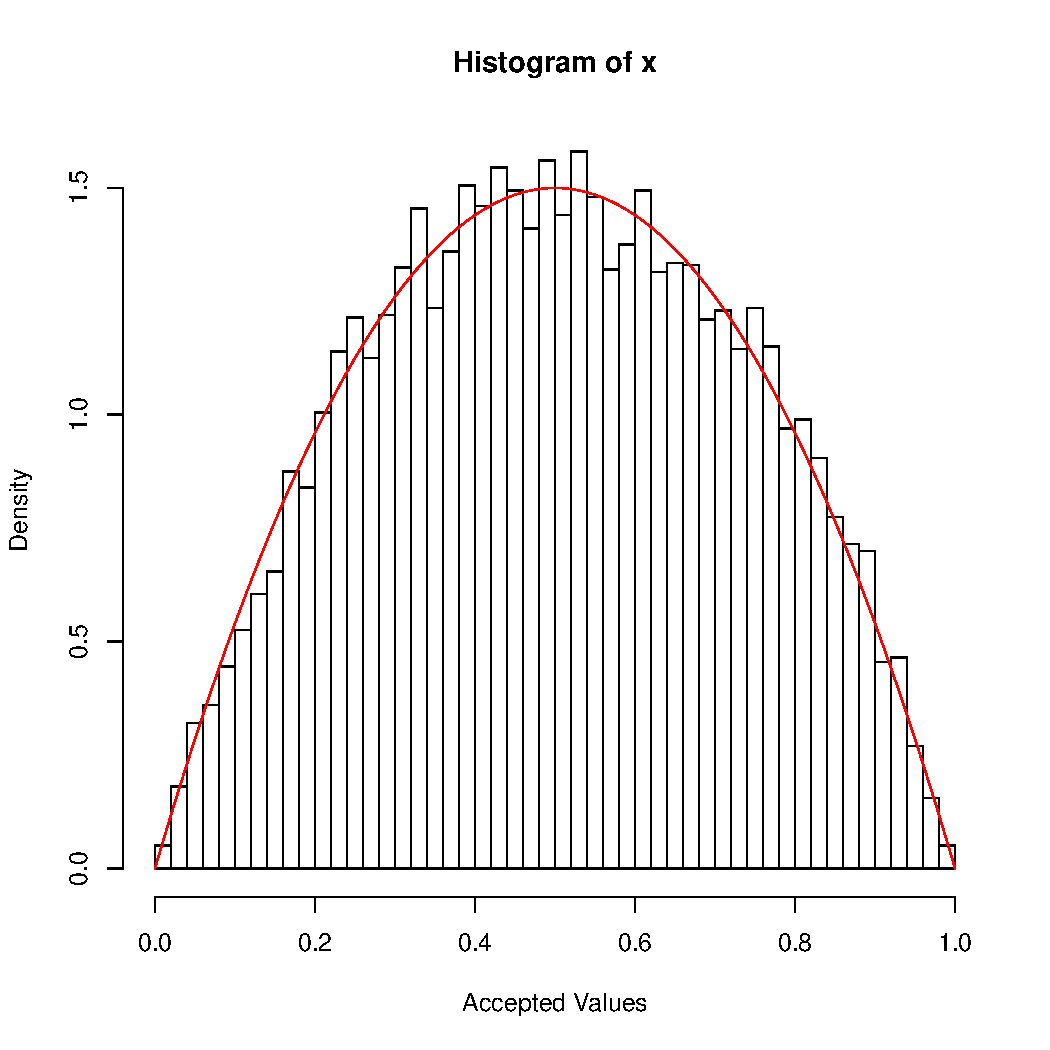
\includegraphics[width=0.60\linewidth]{figure/unnamed-chunk-4-1} 

\end{knitrout}
\subsection*{Part B}
\begin{knitrout}
\definecolor{shadecolor}{rgb}{0.969, 0.969, 0.969}\color{fgcolor}\begin{kframe}
\begin{alltt}
\hlkwd{plot}\hlstd{(}\hlkwd{quantile}\hlstd{(x,} \hlkwc{probs} \hlstd{=} \hlkwd{seq}\hlstd{(}\hlnum{0}\hlstd{,}\hlnum{1}\hlstd{,} \hlkwc{by} \hlstd{=} \hlnum{0.01}\hlstd{)),} \hlkwd{qbeta}\hlstd{(}\hlkwd{seq}\hlstd{(}\hlnum{0}\hlstd{,}\hlnum{1}\hlstd{,}\hlkwc{by} \hlstd{=} \hlnum{.01}\hlstd{),}\hlnum{2}\hlstd{,}\hlnum{2}\hlstd{),}
     \hlkwc{xlab} \hlstd{=} \hlstr{"empirical"}\hlstd{,} \hlkwc{ylab} \hlstd{=} \hlstr{"theortical"}\hlstd{)}
\hlkwd{abline}\hlstd{(}\hlkwc{b}\hlstd{=}\hlnum{1}\hlstd{,}\hlkwc{a}\hlstd{=}\hlnum{0}\hlstd{,} \hlkwc{col} \hlstd{=} \hlstr{"red"}\hlstd{)}
\end{alltt}
\end{kframe}
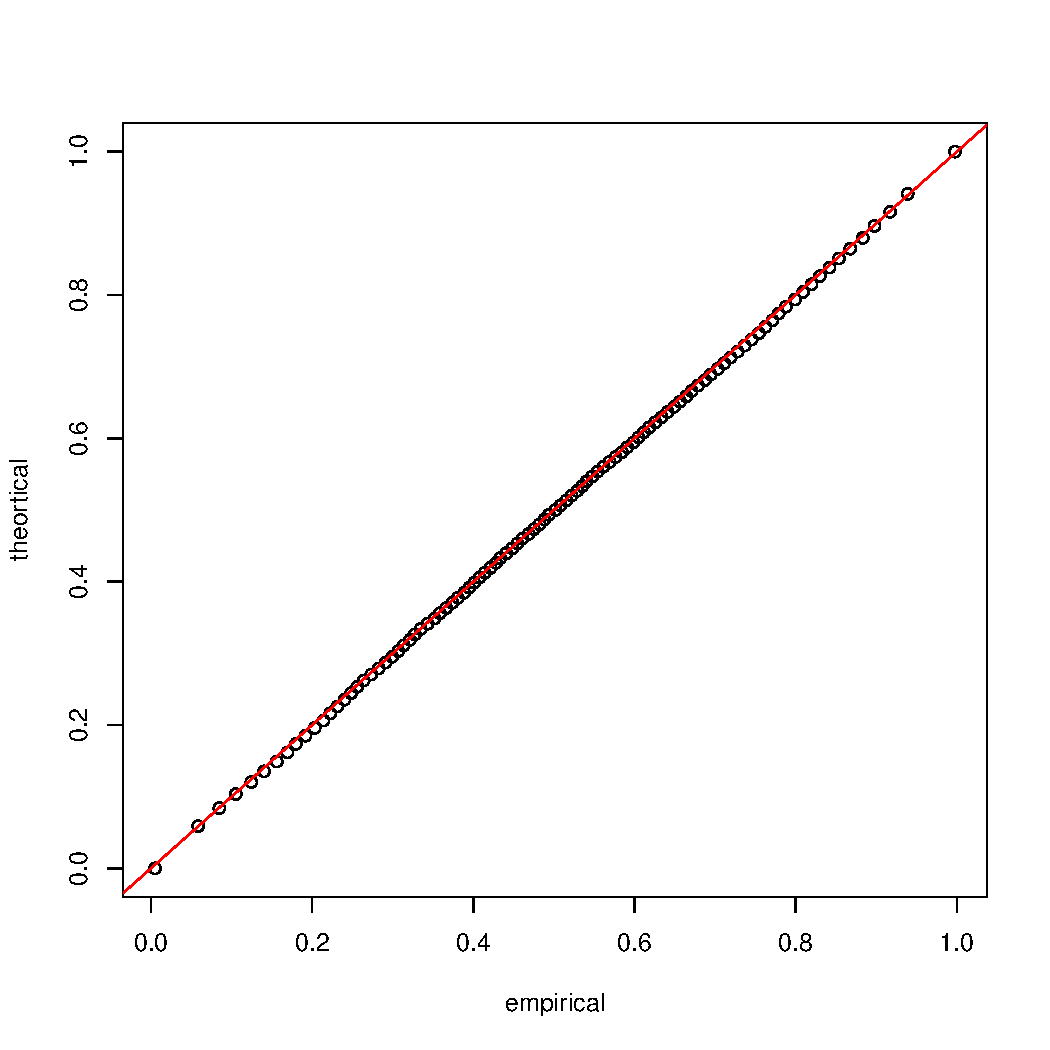
\includegraphics[width=0.60\linewidth]{figure/unnamed-chunk-5-1} 

\end{knitrout}
based on the Q-Q plot, there looks to be a linear relationship between the quantiles of the empirical and theortical values with a slope of 1 and intercept of 0. This indicates that the distribution of both is the same. This observation is further back by the relationship of the histogram to the plot of the density curve.  
\section*{Exercise 5}
\begin{knitrout}
\definecolor{shadecolor}{rgb}{0.969, 0.969, 0.969}\color{fgcolor}\begin{kframe}
\begin{alltt}
\hlkwd{library}\hlstd{(smoothmest)}
\end{alltt}


{\ttfamily\noindent\itshape\color{messagecolor}{\#\# Loading required package: MASS}}\begin{alltt}
\hlstd{M} \hlkwb{=} \hlnum{2}\hlopt{/}\hlkwd{sqrt}\hlstd{(}\hlnum{2}\hlopt{*}\hlstd{pi)}\hlopt{*}\hlkwd{exp}\hlstd{(}\hlnum{.5}\hlstd{)} \hlcom{#note M can be approximated by doing optimize(f=function(x)\{dnorm(x,0,1)/ddoublex(x)\}, interval=c(0,1),maximum =T)$objective}
\hlstd{f} \hlkwb{=} \hlkwa{function}\hlstd{(}\hlkwc{x}\hlstd{)} \hlkwd{dnorm}\hlstd{(x,} \hlnum{0}\hlstd{,} \hlnum{1}\hlstd{)}
\hlstd{g} \hlkwb{=} \hlkwa{function}\hlstd{(}\hlkwc{x}\hlstd{)} \hlkwd{ddoublex}\hlstd{(x)}
\hlstd{Nsim}\hlkwb{=}\hlnum{1e3}
\hlstd{x_rs} \hlkwb{=} \hlkwd{c}\hlstd{()}
\hlstd{count} \hlkwb{=} \hlnum{0}
\hlkwa{while}\hlstd{(}\hlkwd{length}\hlstd{(x_rs)}\hlopt{<}\hlstd{Nsim)\{}
  \hlstd{x} \hlkwb{=} \hlkwd{rdoublex}\hlstd{(}\hlnum{1}\hlstd{); u} \hlkwb{=} \hlkwd{runif}\hlstd{(}\hlnum{1}\hlstd{)}
  \hlstd{count} \hlkwb{=} \hlstd{count} \hlopt{+} \hlnum{1}
  \hlkwa{if}\hlstd{(u} \hlopt{<} \hlkwd{f}\hlstd{(x)}\hlopt{/}\hlstd{(M}\hlopt{*}\hlkwd{g}\hlstd{(x))) \{}
    \hlstd{x_rs}\hlkwb{=} \hlkwd{c}\hlstd{(x_rs,x)}
    \hlstd{\}}
\hlstd{\}}
\hlkwd{hist}\hlstd{(x_rs,} \hlkwc{breaks} \hlstd{=} \hlnum{40}\hlstd{,} \hlkwc{freq} \hlstd{= F)}
\hlkwd{curve}\hlstd{(}\hlkwd{dnorm}\hlstd{(x,} \hlnum{0}\hlstd{,}\hlnum{1}\hlstd{),} \hlkwc{add} \hlstd{= T,} \hlkwc{col} \hlstd{=} \hlstr{"red"}\hlstd{)}
\end{alltt}
\end{kframe}
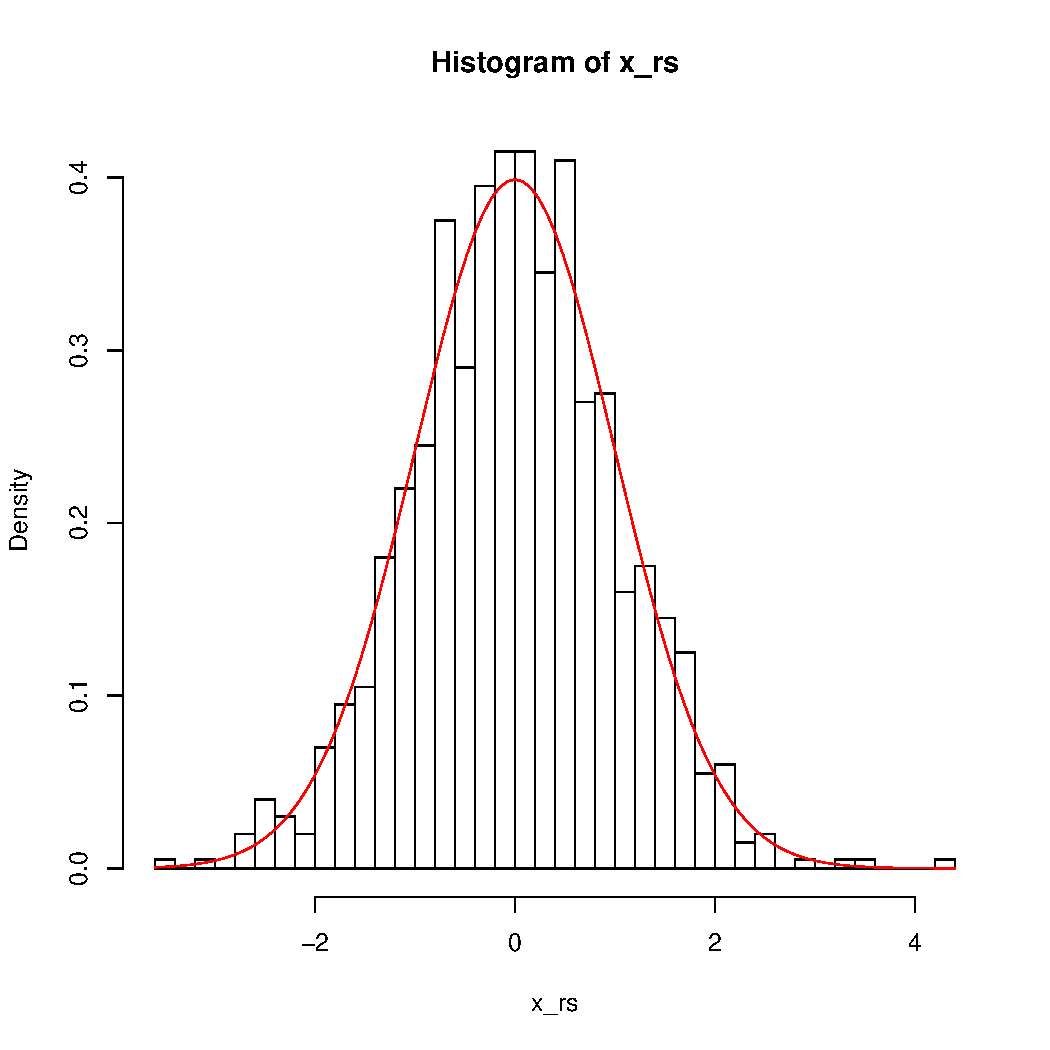
\includegraphics[width=0.60\linewidth]{figure/unnamed-chunk-6-1} 

\end{knitrout}
\end{document}
